\documentclass[11pt]{article}
\usepackage[a4paper,top=16mm,bottom=18mm,left=16mm,right=16mm]{geometry}
\usepackage{kotex}
\usepackage{amsmath,amssymb,mathtools}
\usepackage{array,booktabs,enumitem,fancyhdr,needspace,tabularx,tikz,xcolor}
\usetikzlibrary{arrows.meta,calc,positioning}
\setlength{\parindent}{0pt}
\setlength{\parskip}{0.45em}
\pagestyle{fancy}
\fancyhf{}
\lhead{\textbf{ 2028 CSAT Mathematics MVP }}
\rhead{\small 수학 문제지}
\cfoot{\thepage}

\newcommand{\scorebox}[1]{\fcolorbox{black}{gray!8}{\rule{0pt}{1.8ex}\hspace{0.5em}\textbf{#1점}\hspace{0.5em}}}
\begin{document}
\begin{center}
  {\LARGE\bfseries 2028 CSAT Mathematics MVP}\\[0.5em]
  {\large 시험 시간 100분 \quad 만점 100점}
\end{center}
\vspace{0.4em}
\begin{tabularx}{\linewidth}{>{\raggedright\arraybackslash}p{0.31\linewidth} X}
\toprule
문항 구성 & 1번부터 21번까지는 5지선다형, 22번부터 30번까지는 단답형이다.\\
출제 범위 & 대수, 미적분Ⅰ, 확률과 통계 범위 안에서 구성한 중립적 레이아웃의 시험지다.\\
\bottomrule
\end{tabularx}
\vspace{0.5em}
\textit{참고: topic coverage \{"algebra": 10, "calculus\_1": 10, "probability\_statistics": 10\} \quad difficulty curve basic,basic,basic,basic,basic,standard,standard,standard,standard,standard,standard,standard,standard,standard,challenging,challenging,challenging,challenging,challenging,challenging,challenging,challenging,challenging,advanced,advanced,advanced,advanced,advanced,advanced,advanced}
\vspace{0.6em}
\needspace{12\baselineskip}
\textbf{문항 1.} \hfill \scorebox{ 2 }\\
다항식 및 방정식 기본 이해을 평가하는 모의 문항 1번이다.\\
\begin{enumerate}[label=\arabic*), leftmargin=2.2em, itemsep=0.25em, topsep=0.35em]
\item 4
\item 5
\item 6
\item 7
\item 8
\end{enumerate}
\vspace{0.7em}
\needspace{12\baselineskip}
\textbf{문항 2.} \hfill \scorebox{ 2 }\\
함수와 수열 기초 적용을 평가하는 모의 문항 2번이다.\\
\begin{center}
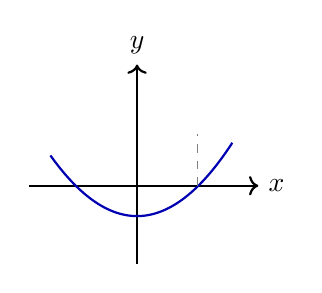
\begin{tikzpicture}[scale=0.55]
  \draw[->, thick] (-2.5,0) -- (2.8,0) node[right] {$x$};
  \draw[->, thick] (0,-1.8) -- (0,2.8) node[above] {$y$};
  \draw[smooth, samples=80, domain=-2:2.2, blue!70!black, thick] plot (\x,{0.35*\x*\x - 0.7});
  \draw[dashed, gray] (1.4,0) -- (1.4,1.2);
\end{tikzpicture}
\end{center}
\begin{enumerate}[label=\arabic*), leftmargin=2.2em, itemsep=0.25em, topsep=0.35em]
\item 8
\item 9
\item 10
\item 11
\item 12
\end{enumerate}
\vspace{0.7em}
\needspace{12\baselineskip}
\textbf{문항 3.} \hfill \scorebox{ 2 }\\
지수로그식 변형을 평가하는 모의 문항 3번이다.\\
\begin{enumerate}[label=\arabic*), leftmargin=2.2em, itemsep=0.25em, topsep=0.35em]
\item 10
\item 11
\item 12
\item 13
\item 14
\end{enumerate}
\vspace{0.7em}
\needspace{12\baselineskip}
\textbf{문항 4.} \hfill \scorebox{ 3 }\\
삼각함수 기본 성질을 평가하는 모의 문항 4번이다.\\
\begin{center}
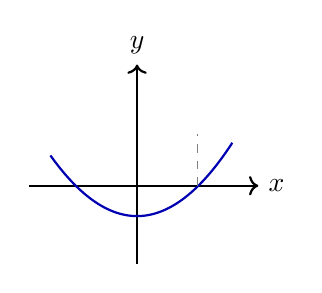
\begin{tikzpicture}[scale=0.55]
  \draw[->, thick] (-2.5,0) -- (2.8,0) node[right] {$x$};
  \draw[->, thick] (0,-1.8) -- (0,2.8) node[above] {$y$};
  \draw[smooth, samples=80, domain=-2:2.2, blue!70!black, thick] plot (\x,{0.35*\x*\x - 0.7});
  \draw[dashed, gray] (1.4,0) -- (1.4,1.2);
\end{tikzpicture}
\end{center}
\begin{enumerate}[label=\arabic*), leftmargin=2.2em, itemsep=0.25em, topsep=0.35em]
\item 14
\item 15
\item 16
\item 17
\item 18
\end{enumerate}
\vspace{0.7em}
\needspace{12\baselineskip}
\textbf{문항 5.} \hfill \scorebox{ 3 }\\
수열의 귀납적 구조 파악을 평가하는 모의 문항 5번이다.\\
\begin{center}
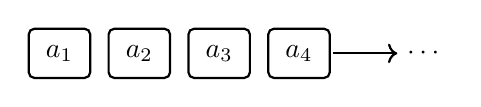
\begin{tikzpicture}[scale=0.78]
  \foreach \x/\v in {0/$a_1$,1.3/$a_2$,2.6/$a_3$,3.9/$a_4$} {
    \draw[rounded corners=2pt, thick] (\x,0) rectangle (\x+1,0.8);
    \node at (\x+0.5,0.4) {\v};
  }
  \draw[->, thick] (4.95,0.4) -- (6.0,0.4);
  \node[right] at (6.0,0.4) {$\cdots$};
\end{tikzpicture}
\end{center}
\begin{enumerate}[label=\arabic*), leftmargin=2.2em, itemsep=0.25em, topsep=0.35em]
\item 17
\item 18
\item 19
\item 20
\item 21
\end{enumerate}
\vspace{0.7em}
\needspace{12\baselineskip}
\textbf{문항 6.} \hfill \scorebox{ 3 }\\
함수의 그래프 해석을 평가하는 모의 문항 6번이다.\\
\begin{center}
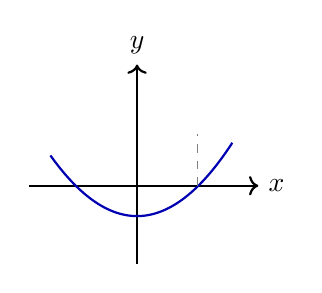
\begin{tikzpicture}[scale=0.55]
  \draw[->, thick] (-2.5,0) -- (2.8,0) node[right] {$x$};
  \draw[->, thick] (0,-1.8) -- (0,2.8) node[above] {$y$};
  \draw[smooth, samples=80, domain=-2:2.2, blue!70!black, thick] plot (\x,{0.35*\x*\x - 0.7});
  \draw[dashed, gray] (1.4,0) -- (1.4,1.2);
\end{tikzpicture}
\end{center}
\begin{enumerate}[label=\arabic*), leftmargin=2.2em, itemsep=0.25em, topsep=0.35em]
\item 19
\item 20
\item 21
\item 22
\item 23
\end{enumerate}
\vspace{0.7em}
\needspace{12\baselineskip}
\textbf{문항 7.} \hfill \scorebox{ 3 }\\
방정식과 부등식 결합을 평가하는 모의 문항 7번이다.\\
\begin{enumerate}[label=\arabic*), leftmargin=2.2em, itemsep=0.25em, topsep=0.35em]
\item 22
\item 23
\item 24
\item 25
\item 26
\end{enumerate}
\vspace{0.7em}
\needspace{12\baselineskip}
\textbf{문항 8.} \hfill \scorebox{ 3 }\\
지수로그함수 실전 적용을 평가하는 모의 문항 8번이다.\\
\begin{enumerate}[label=\arabic*), leftmargin=2.2em, itemsep=0.25em, topsep=0.35em]
\item 26
\item 27
\item 28
\item 29
\item 30
\end{enumerate}
\vspace{0.7em}
\needspace{12\baselineskip}
\textbf{문항 9.} \hfill \scorebox{ 3 }\\
수열 합 계산을 평가하는 모의 문항 9번이다.\\
\begin{center}
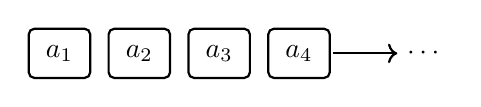
\begin{tikzpicture}[scale=0.78]
  \foreach \x/\v in {0/$a_1$,1.3/$a_2$,2.6/$a_3$,3.9/$a_4$} {
    \draw[rounded corners=2pt, thick] (\x,0) rectangle (\x+1,0.8);
    \node at (\x+0.5,0.4) {\v};
  }
  \draw[->, thick] (4.95,0.4) -- (6.0,0.4);
  \node[right] at (6.0,0.4) {$\cdots$};
\end{tikzpicture}
\end{center}
\begin{enumerate}[label=\arabic*), leftmargin=2.2em, itemsep=0.25em, topsep=0.35em]
\item 29
\item 30
\item 31
\item 32
\item 33
\end{enumerate}
\vspace{0.7em}
\needspace{12\baselineskip}
\textbf{문항 10.} \hfill \scorebox{ 3 }\\
삼각함수 그래프 변환을 평가하는 모의 문항 10번이다.\\
\begin{center}
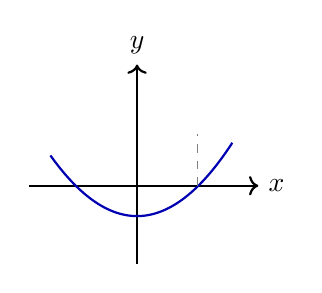
\begin{tikzpicture}[scale=0.55]
  \draw[->, thick] (-2.5,0) -- (2.8,0) node[right] {$x$};
  \draw[->, thick] (0,-1.8) -- (0,2.8) node[above] {$y$};
  \draw[smooth, samples=80, domain=-2:2.2, blue!70!black, thick] plot (\x,{0.35*\x*\x - 0.7});
  \draw[dashed, gray] (1.4,0) -- (1.4,1.2);
\end{tikzpicture}
\end{center}
\begin{enumerate}[label=\arabic*), leftmargin=2.2em, itemsep=0.25em, topsep=0.35em]
\item 31
\item 32
\item 33
\item 34
\item 35
\end{enumerate}
\vspace{0.7em}
\needspace{12\baselineskip}
\textbf{문항 11.} \hfill \scorebox{ 3 }\\
극한의 기본 계산을 평가하는 모의 문항 11번이다.\\
\begin{enumerate}[label=\arabic*), leftmargin=2.2em, itemsep=0.25em, topsep=0.35em]
\item 35
\item 36
\item 37
\item 38
\item 39
\end{enumerate}
\vspace{0.7em}
\needspace{12\baselineskip}
\textbf{문항 12.} \hfill \scorebox{ 3 }\\
연속성 판단을 평가하는 모의 문항 12번이다.\\
\begin{enumerate}[label=\arabic*), leftmargin=2.2em, itemsep=0.25em, topsep=0.35em]
\item 37
\item 38
\item 39
\item 40
\item 41
\end{enumerate}
\vspace{0.7em}
\needspace{12\baselineskip}
\textbf{문항 13.} \hfill \scorebox{ 3 }\\
도함수 해석을 평가하는 모의 문항 13번이다.\\
\begin{center}
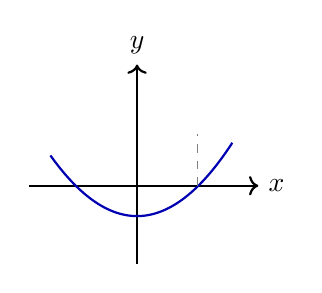
\begin{tikzpicture}[scale=0.55]
  \draw[->, thick] (-2.5,0) -- (2.8,0) node[right] {$x$};
  \draw[->, thick] (0,-1.8) -- (0,2.8) node[above] {$y$};
  \draw[smooth, samples=80, domain=-2:2.2, blue!70!black, thick] plot (\x,{0.35*\x*\x - 0.7});
  \draw[dashed, gray] (1.4,0) -- (1.4,1.2);
\end{tikzpicture}
\end{center}
\begin{enumerate}[label=\arabic*), leftmargin=2.2em, itemsep=0.25em, topsep=0.35em]
\item 40
\item 41
\item 42
\item 43
\item 44
\end{enumerate}
\vspace{0.7em}
\needspace{12\baselineskip}
\textbf{문항 14.} \hfill \scorebox{ 3 }\\
증가감소 구간 파악을 평가하는 모의 문항 14번이다.\\
\begin{center}
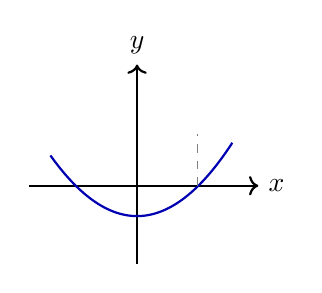
\begin{tikzpicture}[scale=0.55]
  \draw[->, thick] (-2.5,0) -- (2.8,0) node[right] {$x$};
  \draw[->, thick] (0,-1.8) -- (0,2.8) node[above] {$y$};
  \draw[smooth, samples=80, domain=-2:2.2, blue!70!black, thick] plot (\x,{0.35*\x*\x - 0.7});
  \draw[dashed, gray] (1.4,0) -- (1.4,1.2);
\end{tikzpicture}
\end{center}
\begin{enumerate}[label=\arabic*), leftmargin=2.2em, itemsep=0.25em, topsep=0.35em]
\item 44
\item 45
\item 46
\item 47
\item 48
\end{enumerate}
\vspace{0.7em}
\needspace{12\baselineskip}
\textbf{문항 15.} \hfill \scorebox{ 3 }\\
극대극소 조건 해석을 평가하는 모의 문항 15번이다.\\
\begin{center}
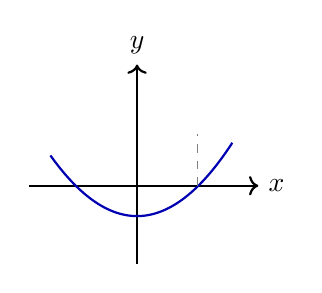
\begin{tikzpicture}[scale=0.55]
  \draw[->, thick] (-2.5,0) -- (2.8,0) node[right] {$x$};
  \draw[->, thick] (0,-1.8) -- (0,2.8) node[above] {$y$};
  \draw[smooth, samples=80, domain=-2:2.2, blue!70!black, thick] plot (\x,{0.35*\x*\x - 0.7});
  \draw[dashed, gray] (1.4,0) -- (1.4,1.2);
\end{tikzpicture}
\end{center}
\begin{enumerate}[label=\arabic*), leftmargin=2.2em, itemsep=0.25em, topsep=0.35em]
\item 47
\item 48
\item 49
\item 50
\item 51
\end{enumerate}
\vspace{0.7em}
\needspace{12\baselineskip}
\textbf{문항 16.} \hfill \scorebox{ 3 }\\
정적분 기초 활용을 평가하는 모의 문항 16번이다.\\
\begin{center}
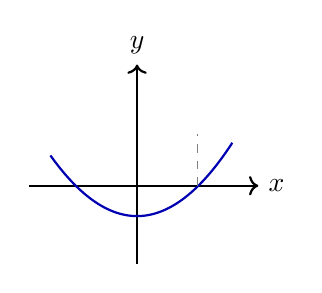
\begin{tikzpicture}[scale=0.55]
  \draw[->, thick] (-2.5,0) -- (2.8,0) node[right] {$x$};
  \draw[->, thick] (0,-1.8) -- (0,2.8) node[above] {$y$};
  \draw[smooth, samples=80, domain=-2:2.2, blue!70!black, thick] plot (\x,{0.35*\x*\x - 0.7});
  \draw[dashed, gray] (1.4,0) -- (1.4,1.2);
\end{tikzpicture}
\end{center}
\begin{enumerate}[label=\arabic*), leftmargin=2.2em, itemsep=0.25em, topsep=0.35em]
\item 49
\item 50
\item 51
\item 52
\item 53
\end{enumerate}
\vspace{0.7em}
\needspace{12\baselineskip}
\textbf{문항 17.} \hfill \scorebox{ 3 }\\
함수와 미분 결합 추론을 평가하는 모의 문항 17번이다.\\
\begin{center}
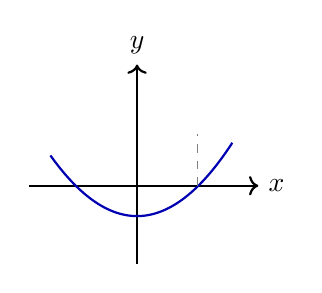
\begin{tikzpicture}[scale=0.55]
  \draw[->, thick] (-2.5,0) -- (2.8,0) node[right] {$x$};
  \draw[->, thick] (0,-1.8) -- (0,2.8) node[above] {$y$};
  \draw[smooth, samples=80, domain=-2:2.2, blue!70!black, thick] plot (\x,{0.35*\x*\x - 0.7});
  \draw[dashed, gray] (1.4,0) -- (1.4,1.2);
\end{tikzpicture}
\end{center}
\begin{enumerate}[label=\arabic*), leftmargin=2.2em, itemsep=0.25em, topsep=0.35em]
\item 52
\item 53
\item 54
\item 55
\item 56
\end{enumerate}
\vspace{0.7em}
\needspace{12\baselineskip}
\textbf{문항 18.} \hfill \scorebox{ 4 }\\
적분과 넓이 계산을 평가하는 모의 문항 18번이다.\\
\begin{center}
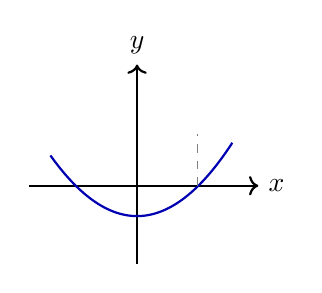
\begin{tikzpicture}[scale=0.55]
  \draw[->, thick] (-2.5,0) -- (2.8,0) node[right] {$x$};
  \draw[->, thick] (0,-1.8) -- (0,2.8) node[above] {$y$};
  \draw[smooth, samples=80, domain=-2:2.2, blue!70!black, thick] plot (\x,{0.35*\x*\x - 0.7});
  \draw[dashed, gray] (1.4,0) -- (1.4,1.2);
\end{tikzpicture}
\end{center}
\begin{enumerate}[label=\arabic*), leftmargin=2.2em, itemsep=0.25em, topsep=0.35em]
\item 56
\item 57
\item 58
\item 59
\item 60
\end{enumerate}
\vspace{0.7em}
\needspace{12\baselineskip}
\textbf{문항 19.} \hfill \scorebox{ 4 }\\
복합 함수 미분 추론을 평가하는 모의 문항 19번이다.\\
\begin{center}
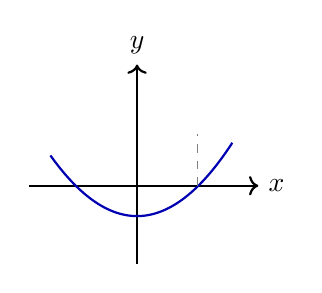
\begin{tikzpicture}[scale=0.55]
  \draw[->, thick] (-2.5,0) -- (2.8,0) node[right] {$x$};
  \draw[->, thick] (0,-1.8) -- (0,2.8) node[above] {$y$};
  \draw[smooth, samples=80, domain=-2:2.2, blue!70!black, thick] plot (\x,{0.35*\x*\x - 0.7});
  \draw[dashed, gray] (1.4,0) -- (1.4,1.2);
\end{tikzpicture}
\end{center}
\begin{enumerate}[label=\arabic*), leftmargin=2.2em, itemsep=0.25em, topsep=0.35em]
\item 58
\item 59
\item 60
\item 61
\item 62
\end{enumerate}
\vspace{0.7em}
\needspace{12\baselineskip}
\textbf{문항 20.} \hfill \scorebox{ 4 }\\
매개 조건 포함 최적화을 평가하는 모의 문항 20번이다.\\
\begin{enumerate}[label=\arabic*), leftmargin=2.2em, itemsep=0.25em, topsep=0.35em]
\item 61
\item 62
\item 63
\item 64
\item 65
\end{enumerate}
\vspace{0.7em}
\needspace{12\baselineskip}
\textbf{문항 21.} \hfill \scorebox{ 4 }\\
경우의 수와 확률 결합을 평가하는 모의 문항 21번이다.\\
\begin{center}
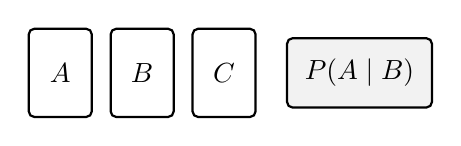
\begin{tikzpicture}[scale=0.8]
  \draw[rounded corners=2pt, thick] (0,0) rectangle (1,1.4);
  \draw[rounded corners=2pt, thick] (1.3,0) rectangle (2.3,1.4);
  \draw[rounded corners=2pt, thick] (2.6,0) rectangle (3.6,1.4);
  \node at (0.5,0.7) {$A$};
  \node at (1.8,0.7) {$B$};
  \node at (3.1,0.7) {$C$};
  \draw[rounded corners=2pt, thick, fill=gray!10] (4.1,0.15) rectangle (6.4,1.25);
  \node at (5.25,0.7) {$P(A \mid B)$};
\end{tikzpicture}
\end{center}
\begin{enumerate}[label=\arabic*), leftmargin=2.2em, itemsep=0.25em, topsep=0.35em]
\item 64
\item 65
\item 66
\item 67
\item 68
\end{enumerate}
\vspace{0.7em}
\needspace{12\baselineskip}
\textbf{문항 22.} \hfill \scorebox{ 4 }\\
확률 변수 계산을 평가하는 모의 문항 22번이다.\\
\begin{center}
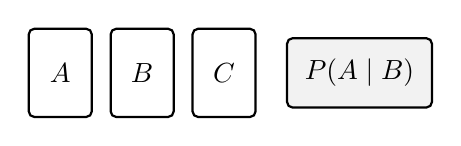
\begin{tikzpicture}[scale=0.8]
  \draw[rounded corners=2pt, thick] (0,0) rectangle (1,1.4);
  \draw[rounded corners=2pt, thick] (1.3,0) rectangle (2.3,1.4);
  \draw[rounded corners=2pt, thick] (2.6,0) rectangle (3.6,1.4);
  \node at (0.5,0.7) {$A$};
  \node at (1.8,0.7) {$B$};
  \node at (3.1,0.7) {$C$};
  \draw[rounded corners=2pt, thick, fill=gray!10] (4.1,0.15) rectangle (6.4,1.25);
  \node at (5.25,0.7) {$P(A \mid B)$};
\end{tikzpicture}
\end{center}
\begin{center}
\fbox{
  \begin{minipage}[c][3.2em][c]{0.62\linewidth}
    \centering \textbf{정답을 자연수로 쓰시오.}
  \end{minipage}
}
\end{center}
\vspace{0.7em}
\needspace{12\baselineskip}
\textbf{문항 23.} \hfill \scorebox{ 4 }\\
조건부확률 적용을 평가하는 모의 문항 23번이다.\\
\begin{center}
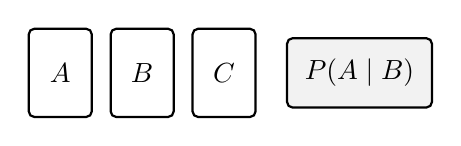
\begin{tikzpicture}[scale=0.8]
  \draw[rounded corners=2pt, thick] (0,0) rectangle (1,1.4);
  \draw[rounded corners=2pt, thick] (1.3,0) rectangle (2.3,1.4);
  \draw[rounded corners=2pt, thick] (2.6,0) rectangle (3.6,1.4);
  \node at (0.5,0.7) {$A$};
  \node at (1.8,0.7) {$B$};
  \node at (3.1,0.7) {$C$};
  \draw[rounded corners=2pt, thick, fill=gray!10] (4.1,0.15) rectangle (6.4,1.25);
  \node at (5.25,0.7) {$P(A \mid B)$};
\end{tikzpicture}
\end{center}
\begin{center}
\fbox{
  \begin{minipage}[c][3.2em][c]{0.62\linewidth}
    \centering \textbf{정답을 자연수로 쓰시오.}
  \end{minipage}
}
\end{center}
\vspace{0.7em}
\needspace{12\baselineskip}
\textbf{문항 24.} \hfill \scorebox{ 4 }\\
분포 해석을 평가하는 모의 문항 24번이다.\\
\begin{center}
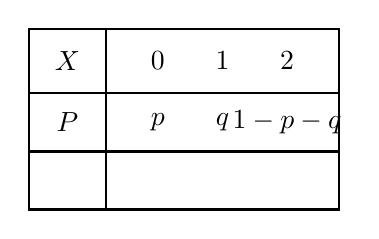
\begin{tikzpicture}[scale=0.82]
  \draw[thick] (0,0) rectangle (4.8,2.8);
  \draw[thick] (1.2,0) -- (1.2,2.8);
  \draw[thick] (0,0.9) -- (4.8,0.9);
  \draw[thick] (0,1.8) -- (4.8,1.8);
  \node at (0.6,2.3) {$X$};
  \node at (2.0,2.3) {$0$};
  \node at (3.0,2.3) {$1$};
  \node at (4.0,2.3) {$2$};
  \node at (0.6,1.35) {$P$};
  \node at (2.0,1.35) {$p$};
  \node at (3.0,1.35) {$q$};
  \node at (4.0,1.35) {$1-p-q$};
\end{tikzpicture}
\end{center}
\begin{center}
\fbox{
  \begin{minipage}[c][3.2em][c]{0.62\linewidth}
    \centering \textbf{정답을 자연수로 쓰시오.}
  \end{minipage}
}
\end{center}
\vspace{0.7em}
\needspace{12\baselineskip}
\textbf{문항 25.} \hfill \scorebox{ 4 }\\
표본평균 계산을 평가하는 모의 문항 25번이다.\\
\begin{center}
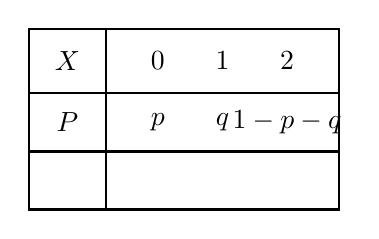
\begin{tikzpicture}[scale=0.82]
  \draw[thick] (0,0) rectangle (4.8,2.8);
  \draw[thick] (1.2,0) -- (1.2,2.8);
  \draw[thick] (0,0.9) -- (4.8,0.9);
  \draw[thick] (0,1.8) -- (4.8,1.8);
  \node at (0.6,2.3) {$X$};
  \node at (2.0,2.3) {$0$};
  \node at (3.0,2.3) {$1$};
  \node at (4.0,2.3) {$2$};
  \node at (0.6,1.35) {$P$};
  \node at (2.0,1.35) {$p$};
  \node at (3.0,1.35) {$q$};
  \node at (4.0,1.35) {$1-p-q$};
\end{tikzpicture}
\end{center}
\begin{center}
\fbox{
  \begin{minipage}[c][3.2em][c]{0.62\linewidth}
    \centering \textbf{정답을 자연수로 쓰시오.}
  \end{minipage}
}
\end{center}
\vspace{0.7em}
\needspace{12\baselineskip}
\textbf{문항 26.} \hfill \scorebox{ 4 }\\
통계량 조건 추론을 평가하는 모의 문항 26번이다.\\
\begin{center}
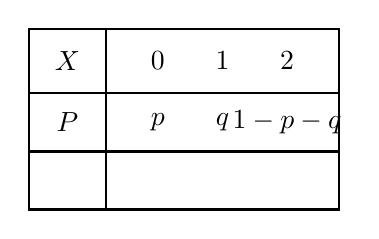
\begin{tikzpicture}[scale=0.82]
  \draw[thick] (0,0) rectangle (4.8,2.8);
  \draw[thick] (1.2,0) -- (1.2,2.8);
  \draw[thick] (0,0.9) -- (4.8,0.9);
  \draw[thick] (0,1.8) -- (4.8,1.8);
  \node at (0.6,2.3) {$X$};
  \node at (2.0,2.3) {$0$};
  \node at (3.0,2.3) {$1$};
  \node at (4.0,2.3) {$2$};
  \node at (0.6,1.35) {$P$};
  \node at (2.0,1.35) {$p$};
  \node at (3.0,1.35) {$q$};
  \node at (4.0,1.35) {$1-p-q$};
\end{tikzpicture}
\end{center}
\begin{center}
\fbox{
  \begin{minipage}[c][3.2em][c]{0.62\linewidth}
    \centering \textbf{정답을 자연수로 쓰시오.}
  \end{minipage}
}
\end{center}
\vspace{0.7em}
\needspace{12\baselineskip}
\textbf{문항 27.} \hfill \scorebox{ 4 }\\
확률분포 함수식 결정을 평가하는 모의 문항 27번이다.\\
\begin{center}
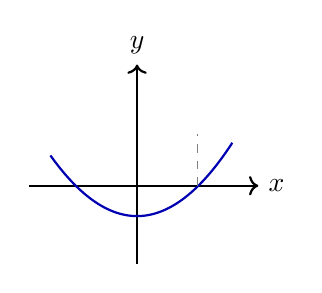
\begin{tikzpicture}[scale=0.55]
  \draw[->, thick] (-2.5,0) -- (2.8,0) node[right] {$x$};
  \draw[->, thick] (0,-1.8) -- (0,2.8) node[above] {$y$};
  \draw[smooth, samples=80, domain=-2:2.2, blue!70!black, thick] plot (\x,{0.35*\x*\x - 0.7});
  \draw[dashed, gray] (1.4,0) -- (1.4,1.2);
\end{tikzpicture}
\end{center}
\begin{center}
\fbox{
  \begin{minipage}[c][3.2em][c]{0.62\linewidth}
    \centering \textbf{정답을 자연수로 쓰시오.}
  \end{minipage}
}
\end{center}
\vspace{0.7em}
\needspace{12\baselineskip}
\textbf{문항 28.} \hfill \scorebox{ 4 }\\
복합 사건의 확률값 산출을 평가하는 모의 문항 28번이다.\\
\begin{center}
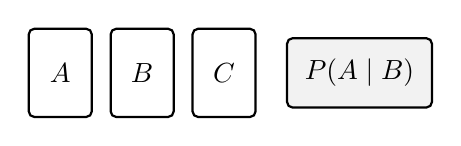
\begin{tikzpicture}[scale=0.8]
  \draw[rounded corners=2pt, thick] (0,0) rectangle (1,1.4);
  \draw[rounded corners=2pt, thick] (1.3,0) rectangle (2.3,1.4);
  \draw[rounded corners=2pt, thick] (2.6,0) rectangle (3.6,1.4);
  \node at (0.5,0.7) {$A$};
  \node at (1.8,0.7) {$B$};
  \node at (3.1,0.7) {$C$};
  \draw[rounded corners=2pt, thick, fill=gray!10] (4.1,0.15) rectangle (6.4,1.25);
  \node at (5.25,0.7) {$P(A \mid B)$};
\end{tikzpicture}
\end{center}
\begin{center}
\fbox{
  \begin{minipage}[c][3.2em][c]{0.62\linewidth}
    \centering \textbf{정답을 자연수로 쓰시오.}
  \end{minipage}
}
\end{center}
\vspace{0.7em}
\needspace{12\baselineskip}
\textbf{문항 29.} \hfill \scorebox{ 4 }\\
통계적 추론 계산을 평가하는 모의 문항 29번이다.\\
\begin{center}
\fbox{
  \begin{minipage}[c][3.2em][c]{0.62\linewidth}
    \centering \textbf{정답을 자연수로 쓰시오.}
  \end{minipage}
}
\end{center}
\vspace{0.7em}
\needspace{12\baselineskip}
\textbf{문항 30.} \hfill \scorebox{ 4 }\\
고난도 통합형 단답 추론을 평가하는 모의 문항 30번이다.\\
\begin{center}
\fbox{
  \begin{minipage}[c][3.2em][c]{0.62\linewidth}
    \centering \textbf{정답을 자연수로 쓰시오.}
  \end{minipage}
}
\end{center}
\vspace{0.7em}
\end{document}
